\section{BÀI TẬP TRẮC NGHIỆM}
% ===================================================================
\begin{ex}
	Một vật rơi có khối lượng $m$, được ném ngang với vận tốc ban đầu $v_0$ ở độ cao $h$. Bỏ qua sức cản của không khí. Thời gian rơi	
	\choice
	{chỉ phụ thuộc vào $m$}
	{\True chỉ phụ thuộc vào $h$}
	{phụ thuộc $v_0$ và $h$}
	{phụ thuộc vào $m$, $v_0$, $h$}
	\loigiai{}
\end{ex}
% ===================================================================
\begin{ex}
	Một vật có khối lượng $m$, được ném ngang với vận tốc ban đầu $v_0$ ở độ cao $h$. Bỏ qua sức cản của không khí. Tầm bay xa của vật phụ thuộc vào
	\choice
	{$m$ và $v_0$}
	{$m$ và $h$}
	{$v_0$ và $h$}
	{$m$, $v_0$ và $h$}
	\loigiai{}
\end{ex}
% ===================================================================
\begin{ex}
	Quỹ đạo chuyển động của vật ném ngang là một 
	\choice
	{đường thẳng}
	{đường tròn}
	{đường xoắn ốc}
	{nhánh parabol}
	\loigiai{}
\end{ex}
% ===================================================================
\begin{ex}
	Quả cầu I có khối lượng  gấp đôi quả cầu II. Cùng một lúc tại độ cao $h$, quả cầu I được thả rơi còn quả cầu II được ném theo phương ngang. Bỏ qua sức cản của không khí. Chọn phát biểu đúng?
	\choice
	{Quả cầu I chạm đất trước}
	{Quả cầu II chạm đất trước}
	{Cả hai quả cầu I và II chạm đất cùng một lúc}
	{Chưa đủ cơ sở để kết luận}
	\loigiai{}
\end{ex}
% ===================================================================
\begin{ex}
	Từ trên một máy bay đang chuyển động đều theo phương ngang người ta thả một vật rơi xuống đất. Bỏ qua sức cản không khí. Nhận xét nào sau đây là \textbf{sai}?	
	\choice
	{Người quan sát đứng trên mặt đất nhìn thấy quỹ đạo của vật là một phần của parabol}
	{Người quan sát đứng trên máy bay nhìn thấy quỹ đạo của vật là một phần của parabol}
	{Người quan sát đứng trên máy bay nhìn thấy quỹ đạo của vật là một đường thẳng đứng}
	{Vị trí chạm đất ở ngay dưới máy bay theo phương thẳng đứng}
	\loigiai{}
\end{ex}
% ===================================================================
\begin{ex}
	Trong chuyển động ném ngang, gia tốc của vật tại một vị trí bất kì luôn có đặc điểm là hướng theo
	\choice
	{phương ngang, cùng chiều chuyển động}
	{phương ngang, ngược chiều chuyển động}
	{phương thẳng đứng, chiều từ dưới lên trên}
	{phương thẳng đứng, chiều từ trên xuống dưới}
	\loigiai{}
\end{ex}
% ===================================================================
\begin{ex}
	Một vật ở độ cao $h$ được ném theo phương ngang với tốc độ $v_0=\SI{50}{\meter/\second}$ và rơi chạm đất sau $\SI{10}{\second}$. Lấy $g=\SI{10}{\meter/\second^2}$. Tầm xa của vật là	
	\choice
	{$\SI{400}{\meter}$}
	{$\SI{200}{\meter}$}
	{$\SI{300}{\meter}$}
	{$\SI{500}{\meter}$}
	\loigiai{}
\end{ex}
% ===================================================================
\begin{ex}
	Ném một vật nhỏ theo phương nằm ngang với tốc độ ban đầu là $\SI{5}{\meter/\second}$, tầm xa của vật là $\SI{15}{\meter}$. Thời gian rơi của vật là
	\choice
	{$\SI{2}{\second}$}
	{$\SI{4}{\second}$}
	{$\SI{1}{\second}$}
	{$\SI{3}{\second}$}
	\loigiai{}
\end{ex}
% ===================================================================
\begin{ex}
	Một vật ở độ cao $h$ được ném theo phương ngang với tốc độ $v_0$ và rơi chạm đất sau $\SI{5}{\second}$. Lấy $g=\SI{10}{\meter/\second^2}$. Vật được ném từ độ cao nào
	\choice
	{\SI{100}{\meter}}
	{\SI{125}{\meter}}
	{\SI{200}{\meter}}
	{\SI{30}{\meter}}
	\loigiai{}
\end{ex}
% ===================================================================
\begin{ex}
	Một quả bóng được ném theo phương ngang với tốc độ ban đầu $v_0=\SI{20}{\meter/\second}$ và rơi xuống đất sau $\SI{3}{\second}$. Lấy $g=\SI{10}{\meter/\second^2}$. Bỏ qua sức cản không khí. Quả bóng được ném từ độ cao
	\choice
	{\SI{45}{\meter}}
	{\SI{30}{\meter}}
	{\SI{60}{\meter}}
	{\SI{90}{\meter}}
	\loigiai{}
\end{ex}
% ===================================================================
\begin{ex}
	Một viên đạn được bắn theo phương ngang từ một khẩu súng đặt ở độ cao $\SI{20}{\meter}$ so với mặt đất. Tốc độ của đạn lúc vừa ra khỏi nòng súng là $\SI{300}{\meter/\second}$. Lấy $g=\SI{10}{\meter/\second^2}$. Điểm đạn rơi xuống cách điểm bắn theo phương ngang là
	\choice
	{\SI{600}{\meter}}
	{\SI{360}{\meter}}
	{\SI{480}{\meter}}
	{\SI{180}{\meter}}
	\loigiai{}
\end{ex}
% ===================================================================
\begin{ex}
	Phương trình quỹ đạo của một vật được ném theo phương ngang có dạng $y=x^2/10$. Lấy $g=\SI{9.8}{\meter/\second^2}$. Tốc độ ban đầu của vật là 
	\choice
	{\SI{7}{\meter/\second}}
	{\SI{5}{\meter/\second}}
	{\SI{2.5}{\meter/\second}}
	{\SI{4.9}{\meter/\second}}
	\loigiai{}
\end{ex}
% ===================================================================
\begin{ex}
	Một vật được ném theo phương ngang với tốc độ $v_0=\SI{15}{\meter/\second}$ và rơi chạm đất sau $\SI{2}{\second}$. Lấy $g=\SI{10}{\meter/\second^2}$. Khi chạm đất vật đạt tốc độ
	\choice
	{\SI{25}{\meter/\second}}
	{\SI{15}{\meter/\second}}
	{\SI{20}{\meter/\second}}
	{\SI{35}{\meter/\second}}
	\loigiai{}
\end{ex}
% ===================================================================
\begin{ex}
	Một vật được ném ngang với tốc độ $v_0=\SI{30}{\meter/\second}$, ở độ cao $h=\SI{80}{\meter}$. Lấy $g=\SI{10}{\meter/\second^2}$. Tầm bay xa và tốc độ của vật khi chạm đất là	
	\choice
	{\SI{120}{\meter}; \SI{50}{\meter/\second}}
	{\SI{50}{\meter}; \SI{120}{\meter/\second}}
	{\SI{120}{\meter}; \SI{70}{\meter/\second}}
	{\SI{70}{\meter}; \SI{120}{\meter/\second}}
	\loigiai{}
\end{ex}
% ===================================================================
\begin{ex}
	Một vật được ném theo phương ngang với tốc độ ban đầu $v_0=\SI{8}{\meter/\second}$. Lấy $g=\SI{10}{\meter/\second^2}$. Sau khi ném $\SI{2}{\second}$, phương của vận tốc và phương ngang hợp nhau một góc 	
	\choice
	{\SI{37.5}{\degree}}
	{\SI{84.7}{\degree}}
	{\SI{62.8}{\degree}}
	{\SI{68.2}{\degree}}
	\loigiai{}
\end{ex}
\section{BÀI TẬP TỰ LUẬN}
% ======================================================================
\begin{ex}
	Từ độ cao $\SI{45}{\meter}$ so với mặt đất, một vật được ném theo phương ngang với vận tốc đầu $v_0$. Khi chạm đất, vector vận tốc của vật hợp với phương ngang góc $\SI{30}{\degree}$. Tìm $v_0$ và tầm xa vật đạt được. Lấy $g=\SI{9.8}{\meter/\second^2}$.
	\loigiai{$v_0=\xsi{30\sqrt{3}}{\meter/\second}$; $L=\SI{156}{\meter}$.} 
\end{ex}
% ======================================================================
\begin{ex}
	Một người trượt tuyết rời khỏi đường trượt theo phương ngang với vận tốc $\SI{25}{\meter/\second}$. Người này đáp xuống một dốc nghiêng $\SI{35}{\degree}$ so với phương ngang ở vị trí cách điểm xuất phát bao xa? Lấy $g=\SI{9.8}{\meter/\second^2}$.
	\loigiai{$d=\SI{109}{\meter}$}
\end{ex}
% ======================================================================
\begin{ex}
	Một quả cầu được ném theo phương ngang từ độ cao $\SI{80}{\meter}$. Sau khi chuyển động được $\SI{3}{\second}$ vận tốc quả cầu hợp với phương ngang góc $\SI{45}{\degree}$. Lấy $g=\SI{10}{\meter/\second^2}$.
	\begin{enumerate}[label=\alph*)]
		\item Tìm tốc độ ban đầu của quả cầu.
		\item Qủa cầu sẽ chạm đất lúc nào? Ở đâu? Với tốc độ bao nhiêu?
	\end{enumerate}	
	\loigiai{
		\begin{enumerate}[label=\alph*)]
			\item $v_0=\SI{30}{\meter/\second}$.
			\item $t=\SI{4}{\second}$; $L=\SI{120}{\meter}$; $v=\SI{50}{\meter/\second}$.
		\end{enumerate}
	}
\end{ex}

% ======================================================================
\begin{ex}
	\immini{Một kiến trúc sư cảnh quan đang lên kế hoạch xây dựng một thác nước nhân tạo trong công viên thành phố. Một kênh dẫn nằm ngang ở độ cao $h=\SI{2.35}{\meter}$ dẫn nước với tốc độ $\SI{1.70}{\meter/\second}$ chảy vào một bể chứa bên dưới như hình vẽ. Lấy $g=\SI{9.8}{\meter/\second^2}$.
		\begin{enumerate}[label=\alph*)]
			\item Tính tầm xa của nước khi đổ xuống bể chứa.
			\item Để bán kế hoạch của mình cho hội đồng thành phố, kiến trúc sư muốn xây dựng một mô hình theo tỷ lệ tiêu chuẩn, có kích thước bằng 1 phần 12 kích thước thật. Nước trong kênh trong mô hình phải chảy với tốc độ bao nhiêu?
	\end{enumerate}	}
	{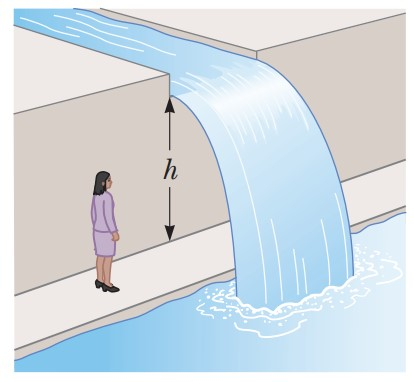
\includegraphics[scale=0.7]{../figs/G10-BTNEMNGANG2}}
	
	\loigiai{}
\end{ex}
% ======================================================================
\begin{ex}
	\immini{Một chiếc xe tải chở đầy dưa hấu dừng lại đột ngột để tránh lao xuống sông do cây cầu đã bị cuốn trôi. Việc dừng xe đột ngột khiến một số quả dưa văng khỏi xe tải. Một quả dưa rời khỏi mui xe tải với tốc độ ban đầu $v_i=\SI{10}{\meter/\second}$ theo phương ngang. Mặt cắt ngang của bờ sông có dạng nửa parabol $y^2=16x$, với đỉnh là vị trí ban đầu của quả dưa hấu và $x,y$ đều đo bằng mét. Quả dưa hấu va vào bờ sông ở tọa độ bằng bao nhiêu?	Lấy $g=\SI{9.8}{\meter/\second^2}$.}
	{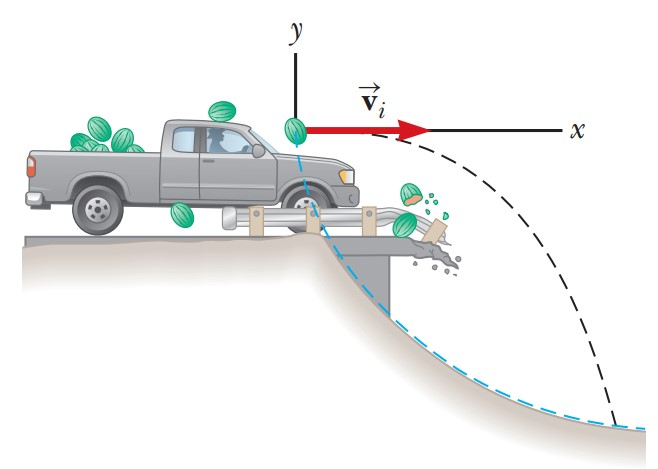
\includegraphics[scale=0.6]{../figs/G10-BTNEMNGANG2-2}}
	\loigiai{}
\end{ex}
% ======================================================================
\begin{ex}
	\immini{Trong hình bên, bốn lá sen nhô lên khỏi mặt nước và một con ếch đang ở ngồi trên bờ hồ. Cho rằng độ cao của bờ hồ và lá sen so với mặt nước lần lượt là $H=6h$, $h_a=h_b=4h$, $h_c=h_d=h$. Ếch và tâm của hai lá sen a, b cùng nằm trên một mặt phẳng thẳng đứng. Giao điểm của thân bốn lá sen với mặt nước là bốn đỉnh của một hình vuông song song với bờ sông và có chiều dài cạnh bằng $\ell$. Khoảng cách theo phương ngang giữa lá sen a và bờ hồ cũng là $\ell$. Xem con ếch chuyển động như vật ném ngang với gia tốc trọng trường $g$.}
	{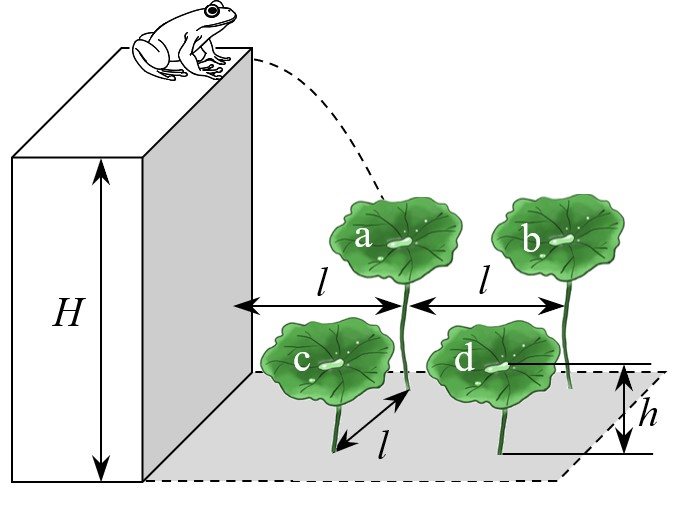
\includegraphics[scale=0.6]{../figs/G10-BTNEMNGANG2-5}}
	\begin{enumerate}[label=\alph*)]
		\item Sau một cú nhảy, con ếch đã đậu thành công trên lá sen a. Tìm tốc độ ban đầu của con ếch.
		\item Tốc độ nhảy ban đầu của con ếch ứng với sự rơi trên lá sen nào là nhỏ nhất? Giải thích một cách tường minh.
	\end{enumerate}
	\loigiai{}
\end{ex}
% ======================================================================
\begin{ex}
	\immini{Chó sói Wile E. Coyote cố gắng một lần nữa để bắt chú gà lôi thông minh Road Runner. Sói Wile E. mang một đôi giày trượt patin trợ lực mới để tạo ra gia tốc không đổi $\SI{15}{\meter/\second^2}$ trên phương ngang như hình bên. Con sói xuất phát từ trạng thái nghỉ cách mép vách đá $\SI{70}{\meter}$ vào thời điểm gà lôi vượt qua nó và lao về hướng vách đá. Lấy $g=\SI{9.8}{\meter/\second^2}$.
		\begin{enumerate}[label=\alph*)]
			\item Nếu gà lôi chạy với tốc độ không đổi, hãy tìm tốc độ tối thiểu của nó để đến được vách đá trước khi con sói bắt kịp.
			\item Nếu vách đá cao $\SI{100}{\meter}$ so với chân núi, hãy tìm nơi con sói rơi xuống. \textit{(Giả sử giày trượt của Wile E. vẫn còn hoạt động khi nó đang bay và thành phần phần gia tốc theo phương ngang anh ta vẫn bằng $\SI{15}{\meter/\second^2}$ không đổi).}
	\end{enumerate}}
	{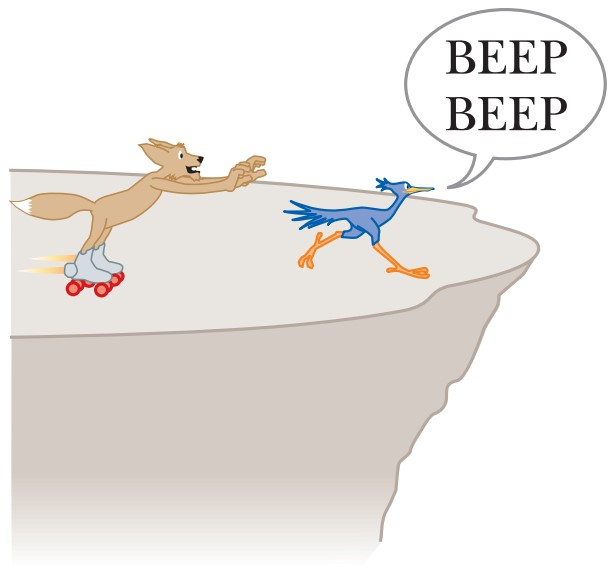
\includegraphics[scale=0.6]{../figs/G10-BTNEMNGANG2-4}}
	
	\loigiai{}
\end{ex}
% ======================================================================
\begin{ex}
	\immini{Một máy bay ném bom, bay theo phương ngang ở độ cao $H=\SI{500}{\meter}$ so với mặt đất, chuyển động nhanh dần đều với gia tốc $a=\SI{2}{\meter/\second^2}$ và các quả bom được thả sau những khoảng thời gian bằng nhau $t=\SI{0.5}{\second}$. Tìm khoảng cách giữa các điểm rơi của quả bom thứ 9 và thứ 11 trên mặt đất nếu quả bom thứ nhất được thả ra khi vận tốc của máy bay là $v_0=\SI{100}{\meter/\second}$. Cho $g=\SI{10}{\meter/\second^2}$ và bỏ qua sức cản của không khí.}
	{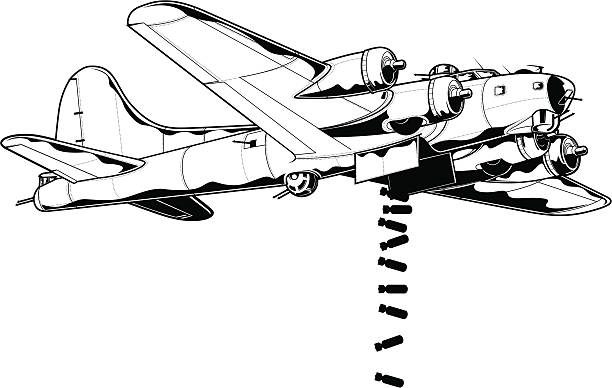
\includegraphics[scale=0.7]{../figs/G10-BTNEMNGANG2-3}}
	\loigiai{$\Delta s=L+s_{11}-s_9=\SI{129}{\meter}$.}
\end{ex}